\section{Trivia Game}

The first modality of the game is a trivia-type game, that will use Romie, the robot in
WebLab-Deusto and its labyrinth to create an experience for learning general knowledge. Moreover,
since the trivia questions will be configurable, so that the game can be adapted.

\subsection{Software and Hardware Requirements}

This software will have tight requirements in terms of user-friendliness, communication stability
and security, since it must be developed using as far as possible current hardware and be easy to
use by young students. Moreover, since it will be presented in crowded events, it must support high
load and availability.

Furthermore, due to the requirements of the project, it must be integrated with the WebLab-Deusto
platform and must be deployable in that environment. Thus, the requirements specification will be
as it follows:

\subsubsection{Software requirements:}

\begin{itemize}
	\item The software must be able to communicate with the robot.
	\item The software must be able to send control commands to the robot.
	\item The software must be able to receive command results from the robot.
	\item The software must be integrated in the WebLab-Deusto platform as a new experiment.
	\item The software must have an easy to use user interface based on human-computer interaction
	principles.
	\item The software must be stable enough to support tens of accesses per hour.
	\item The software must provide enough questions so that the user never finishes with them and
	can be randomly selected.
	\item The game must increase difficulty as the user gets more points.
	\item The game must finish in less than 15 minutes.
	\item A ranking must be provided after finishing the game for the user to know its ranking.
\end{itemize}

\subsubsection{Hardware requirements:}

\begin{itemize}
	\item The hardware must be placed in WebLab-Deusto.
	\item The robot must never get blocked, so in the case of an incident it must be automatically
	recovered.
	\item The cameras must be accessible from the Internet.
	\item The robot must be controlled via Bluetooth.
	\item The robot must never run out of power.
	\item The robot must be able to read all the \acrshort{rfid} tags with at least 99~\% accuracy.
	\item The robot must use the current labyrinth in WebLab-Deusto.
	\item No new hardware can be added to the current WebLab server (Plunder).
\end{itemize}

\subsection{Design Specification}

Taking into account the previous requirements, it has been decided to do a small hardware redesign
and a complete software design for the project. We will now see the hardware and software design
specifications.

\subsubsection{Hardware Specification}

Current robot is deployed with a simple \acrshort{rfid} reader (model ID-12) not capable of reading
further than 120mm~\cite{rfid}, which generates some reading inconsistencies from the distance the
sensor is located in the robot (about 100-120mm from the ground). For that reason, it has been
decided to use a new module, the new module will be model ID-20LA. This will give the robot a much
higher reliability when reading \acrshort{rfid} tags, since the range of the new sensor is
180mm~\cite{rfid}.

On the other hand, there is currently an issue with the availability of the robot. It is powered
with a 2Ah \acrshort{lipo} battery, and is recharged when needed. This has a big issue, since as we
have seen, in high load conditions would not meet the required availability, and furthermore, in
weekends or holidays, we will not be able to change and recharge the battery, so it has been decided
to deploy a cable installation from the roof of the ceiling of the laboratory, and the design of the
robot has been adapted so that the cables do not get stuck in the labyrinth.

The rest of the robot will be used as it is, since it provides with the needed capabilities for the
needs of the project: It has a wall sensor capable of avoiding crashes with walls, infrared sensors
to detect the lines in the ground, motors and wheels capable of moving the robot, Bluetooth
connection to communicate with it and Arduino microcontroller, to install the needed firmware.

The robot is currently configured with a camera {TODO MODEL} that provides infrared vision if the
light is shut down and normal vision if not, and it can be accessed from Wi-Fi and Ethernet. In this
case we will use it via Wi-Fi, since the robot will be moving around a big space.

\subsubsection{Software Specification}

The software in for this implementation will be divided modularly, thinking on scalability and
code reuse. The application must be built on top of WebLab-Deusto, so we will use as much as
possible the provided \acrshort{api}s. Moreover, and due to deployment needs, the software will be
divided between the robot, an intermediate server and WebLab software.

The robot will use a slightly modified version of the current firmware, since we need it not to get
blocked by any wall in case of crash and we need a more reliable implementation. Nevertheless, the
external Bluetooth \acrshort{api} will be the same as the one that was already implemented at the
beginning of the project:

It will provide a ``F'' command to go forward, that will return the \acrshort{rfid} tag if it finds
one, a ``L'' command to turn left, its counterpart ``R'' command to turn right and it will also
provide the command ``S'' that will check if there is a wall in front of the robot. Nevertheless,
and even if the experiment server can check for a wall, the robot itself has been programmed to
return a ``NAK'' command if it is commanded to go forward against a wall.

The robot itself works following the lines in the labyrinth until it finds an intersection. It is
also capable of turning in those intersections, so if it is commanded to turn right, it will perform
a 90 degree turn right and face the path in its right. When the robot stops on top of a
\acrshort{rfid} tag, it will return the tags address.

The intermediate server will provide a small \acrshort{rest} \acrshort{api} in a small Python
server. Its only duty will be to provide a simple interface for the robot using \acrshort{http}
instead of Bluetooth, needed due to deployment constraints. We can see an example of the
\acrshort{api} usage with Python in algorithm~\ref{alg:romie-rasp}.

\begin{center}
\begin{minipage}{.9\textwidth}
\singlespace
\begin{pyglist}[language=python, caption={Romie \acrshort{rest} \acrshort{api} example.},
	label={alg:romie-rasp}, listingname={Algorithm}, numbers=left]
import urllib2

# Let's go forward and get RFID tag if exists
tag = urllib2.urlopen('http://192.168.0.190:8000/f', timeout = 60).read()

# Let's turn left
result = urllib2.urlopen('http://192.168.0.190:8000/l', timeout = 60).read()

# Let's turn right
result = urllib2.urlopen('http://192.168.0.190:8000/r', timeout = 60).read()

# Let's check if we have a wall in front of us
result = urllib2.urlopen('http://192.168.0.190:8000/s', timeout = 60).read()
\end{pyglist}
\end{minipage}
\end{center}

Then, the experiment server required by the WebLab-Deusto architecture, will provide a WebLab
command \acrshort{api}, that will be callable by the client of the experiment. This server will be
developed in Python because the WebLab server libraries are better intended for this language. The
data for the ranking will be stored in a SQLite 3 database. This database provides all the needed
\acrshort{acid} constraints with as little as simple as possible \acrshort{sql}
interface~\cite{sqlite}. It provides all the needed functionality from a \acrshort{rdbms}.

The experiment server \acrshort{api} will have all the needed commands to use the experiment. For
the ones that need data being sent to the server, \acrshort{json} has been used. It is preferred
over \acrshort{xml} due to the higher compatibility of \acrshort{json} and the more data-orientation
of this \acrshort{rfc}. This provides lower overhead~\cite{xml_vs_json}.

\begin{itemize}
	\item ``\textbf{F}'', ``\textbf{L}'' and ``\textbf{R}'' commands, to move forward and turn left
	and right. The ``S'' command is not provided since the experiment does not require it and the
	robot will not drive towards a wall. The ``\textbf{F}'' will return a random question based on
	the current user's points.

	\item ``\textbf{CHECK\_REGISTER}'' command, to check if the user has been registered in the
	experiment before and decide if the experiment should show the registration form.

	\item ``\textbf{REGISTER}'' command, to send the registration data to the server and insert it
	into the SQLite database.

	\item ``\textbf{ANSWER}'' command, to send the answer given by the user to a question. It will
	return the new date for finishing the experiment and the new points for the user. These will not
	change if the answer was not correct.

	\item ``\textbf{FINISH}'' command, to finish the experiment and receive the final ranking.
\end{itemize}

Finally, the client will be developed using \acrshort{html} 5, JavaScript (using JQuery library) and
Bootstrap for a rapid development. It will use the WebLab JavaScript library to communicate with the
experiment server. This library is an asynchronous \acrshort{ajax} library that provides a simple
interface to interact with experiments. We can see an example in algorithm~\ref{alg:weblab-lib}.

\begin{center}
\begin{minipage}{.9\textwidth}
\singlespace
\begin{pyglist}[language=javascript, caption={WebLab JavaScript library example.},
	label={alg:weblab-lib}, listingname={Algorithm}, numbers=left]
// Callback registration that will be
// called after reserving the experiment
Weblab.setOnStartInteractionCallback(start);

// Sending command to the experiment server
Weblab.sendCommand("L", function(response) {
    console.log("Good response: " + response);
}, function(response) {
    console.log("Bad response: " + response);
});
\end{pyglist}
\end{minipage}
\end{center}

TODO: Software design graphic (experiment flow chart)

\subsection{Deployment Considerations}

The deployment must be done in WebLab-Deusto, a remote laboratory environment with three custom
networks and limited physical space. In figure~\ref{fig:weblab-network} we can see the network of
WebLab-Deusto. As we can see, Plunder is the core server. It provides access to WebLab-Deusto web
environment and it provides most of the experiment servers. On the other hand, Blood is the one
working as a proxy for all the cameras in WebLab-Deusto, some of them connected by Wi-Fi and others
by Ethernet.

\begin{figure}[!htbp]
	\centering
	\includegraphics[width=0.9\textwidth]{fig/weblab-network}
	\caption{WebLab-Deusto network simplification.}\label{fig:weblab-network}
\end{figure}

In this case, since we need Bluetooth to connect our experiment server to the robot, and Plunder,
Blood and WebLab-test should not need new hardware, we will use a Raspberry Pi Model B
(figure~\ref{fig:rasp}) with a \acrshort{usb} Bluetooth dongle to connect to the robot and to
provide a simple \acrshort{http} server with the \acrshort{rest} \acrshort{api}. This small computer
provides us with the needed hardware for such small web server, since it provides 512~MB of
\acrshort{ram}, a 700~Mhz \acrshort{arm} \acrshort{cpu}, 2 \acrshort{usb} ports and an Ethernet
port. All this in a small form factor, not bigger than a usual credit card, and consuming only
3.5~W.

\begin{figure}[!htbp]
	\centering
	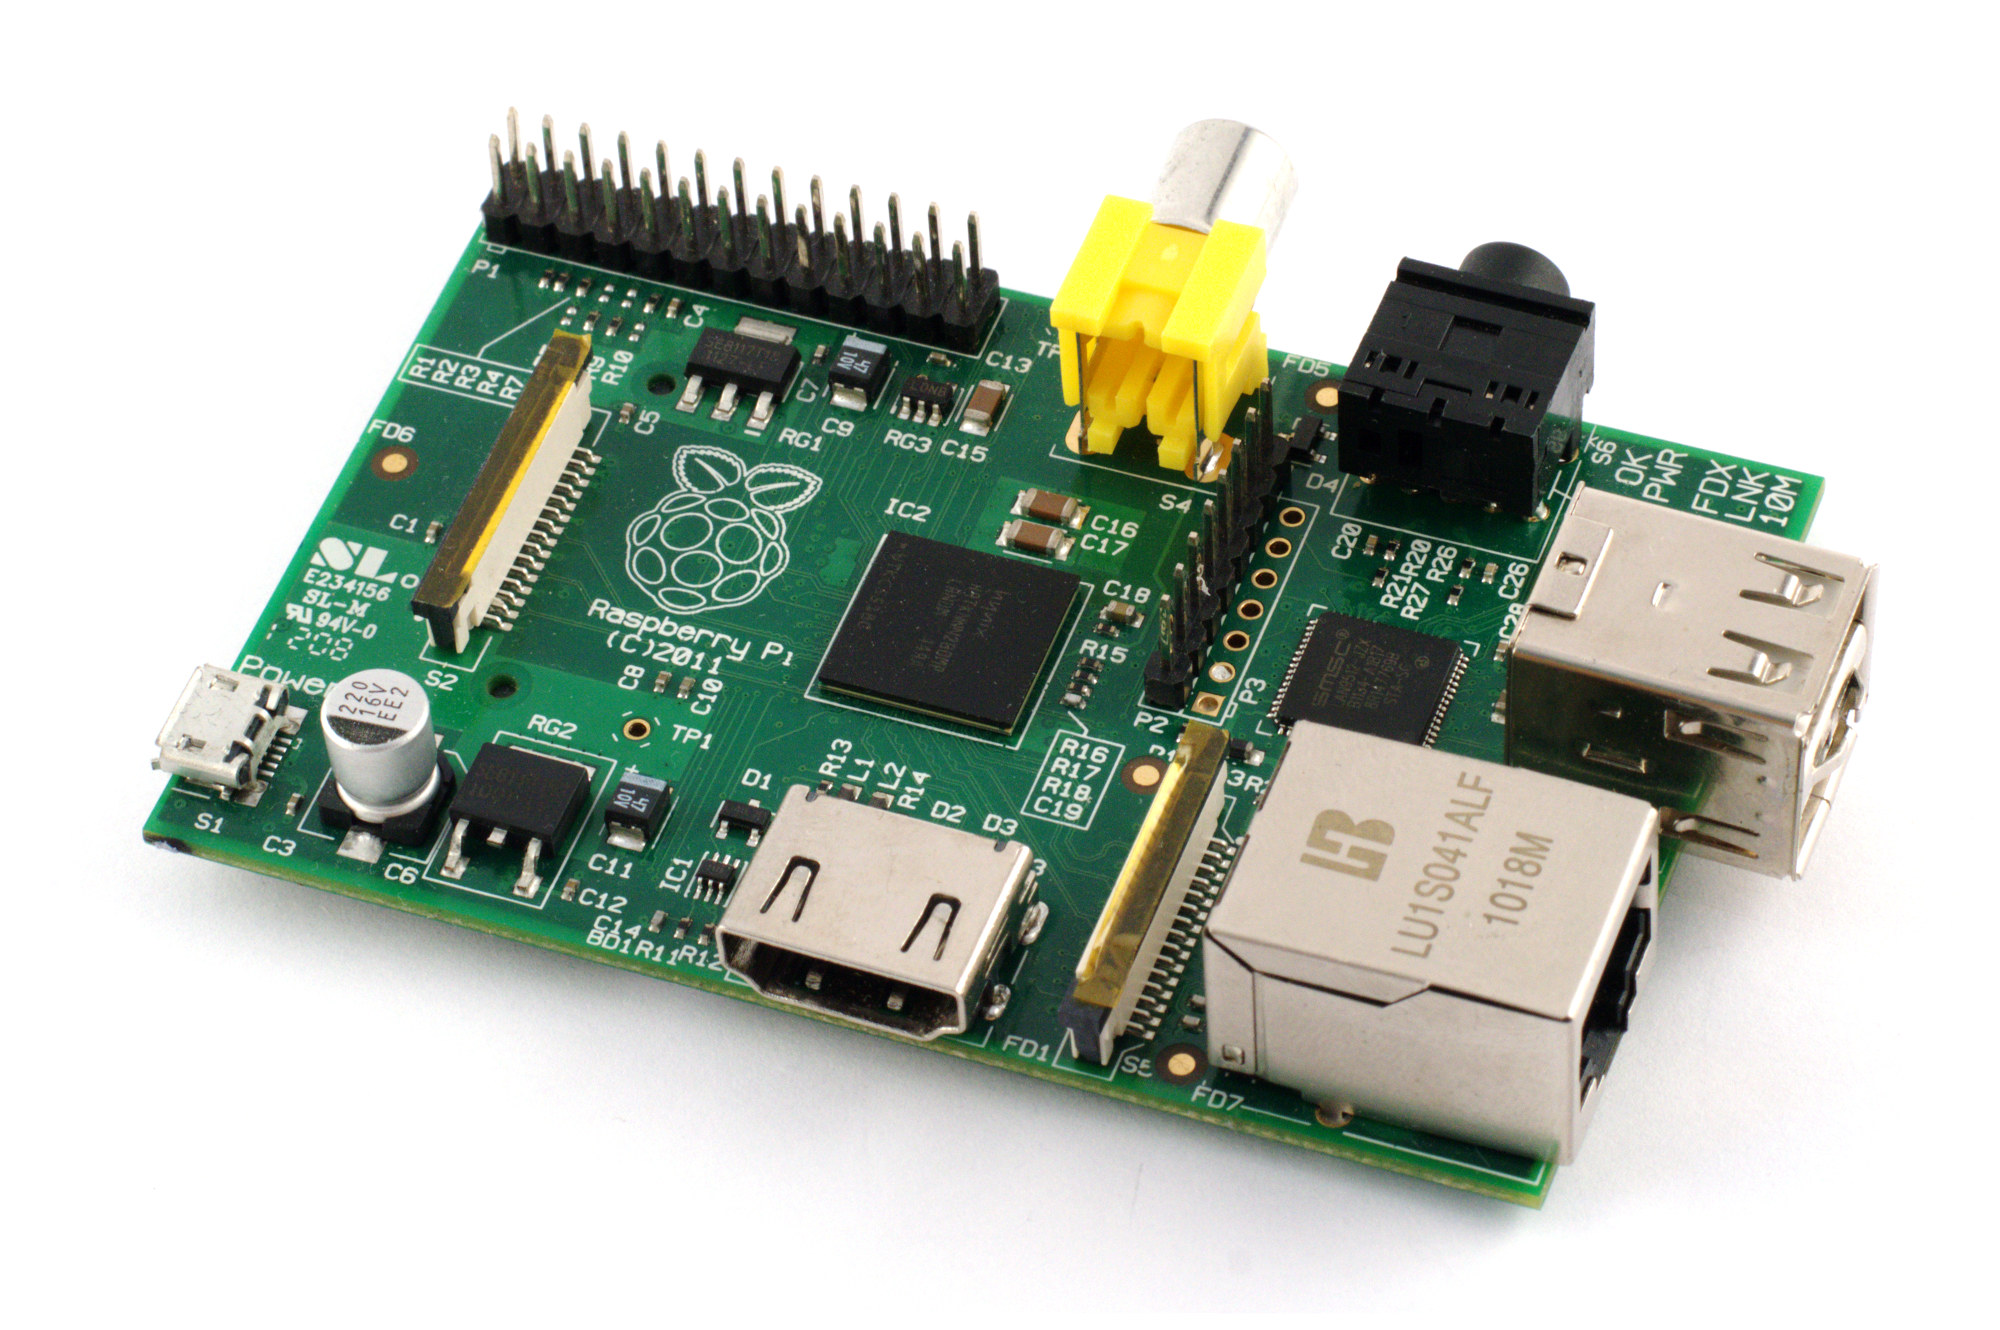
\includegraphics[width=0.7\textwidth]{fig/rasp}
	\caption{Raspberry Pi model B computer.}
	\label{fig:rasp}
\end{figure}

This small computer will be connected via Ethernet to the WebLab network, while two cameras (the top
camera and the on-board camera) will be connected via Wi-Fi to WebLab camera network, using Blood as
the \acrshort{http} proxy server.

Finally, since the server software will change many times during the development, and Plunder must
be restarted for each change if the experiment server is located there, the experiment server for
this experiment will be located in WebLab-test. This way, there will be no need to restart Plunder
each time a new change is made to the experiment, giving higher availability to WebLab-Deusto.

\subsection{Testing Plan}

The testing for this software is divided in 3 main environments. First of all, the usual manual
testing is made by the developers and by the administrators of WebLab-Deusto. This showed many bugs
that we were able to fix almost as soon as they appeared, but in any case, this is not enough
for a production environment.

After the manual testing, WebLab-Deusto has a \acrlong{ci} system connected to Travis \acrshort{ci}
in GitHub. It provides many unit tests that provide stability to the code, since we receive emails
when a commit does not pass the tests. Nevertheless, for \acrshort{gui}, it is difficult to provide
unit tests.

TODO: Forotech testing

\subsection{User Manual}

TODO

\subsection{Issue Management}

TODO: painting the labyrinth,
